\documentclass[12pt]{article}
\usepackage{MinionPro}
\usepackage{CJK}
%\usepackage[scaled=0.85]{beramono}  %%% scaled=0.775
\usepackage[T1]{fontenc}
\usepackage{graphicx,booktabs,tabularx,psfrag}
\usepackage{xcolor}
\usepackage[a4paper]{geometry}
\usepackage{url}

\usepackage{pstool}

\usepackage{graphicx}
\begin{document}
\begin{CJK}{UTF8}{cwmb}
\renewcommand{\figurename}{圖}

\voffset=-1cm
\textwidth=5.6in
\textheight=9.2in

\newenvironment{num}
 {\leftmargini=6mm\leftmarginii=8mm
  \begin{enumerate}\itemsep=-2pt}
 {\end{enumerate}}

\newenvironment{sol}
 {\begin{quote}\mbox{}\llap{\color{blue}{解答:}\rule{10mm}{0pt}}\hspace*{-4pt}}{\end{quote}}


\thispagestyle{empty}
\fontsize{12}{20pt}\selectfont
\begin{center}
{\large\CJKfamily{cwyb}{經濟學原理下, 習題4}}\\[3mm]
劉彥佑 (R99628130)\\
李卿澄 (B97501046)\\
黃博億 (B99101014)\\
王祉婷 (B00704056)
\end{center}

\begin{num}
\item 
	\begin{num}
		\item 甲欲貸出20-15=5,乙欲借入15-15=0。
		\item 實質債券餘額圖:
\begin{figure}[htp]
\centering
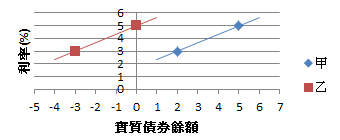
\includegraphics[scale=1.00]{1b.png}
\end{figure} 
		\item 可貸資金市場供需圖:
\begin{figure}[htp]
\centering
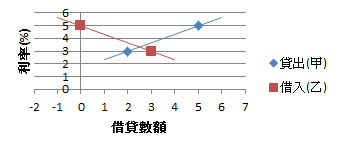
\includegraphics[scale=1.00]{1c.png}
\end{figure} 
		\item 根據上題圖形,可得甲之貸出與乙之借入交於($\frac{5}{2},\frac{10}{3}$),利率為$\frac{10}{3}$之處,高於3\%,小於5\%。
		\item 總和儲蓄=0,因為甲之儲蓄全部都借給了乙,滿足乙之負儲蓄。
		\item 當利率為5\%時總產出為35,利率3\%時為31,可以發現利率越低總產出越低,而可貸資金市場達成均衡時之利率介於3\%至5\%之間,總產出也應介於31至35之間,不會高過35。
		\item 利率為5\%時總消費為30,利率3\%總消費為32,當利率越低總消費越高,但可貸資金市場均衡之時利率介在3\%至5\%之間,故總消費也應介於30至32,不會高於32。
	\end{num}
\item 
	\begin{num}
		\item 甲仍為農夫時,均衡利率為5\%,此經濟中之總消費線與總產出線交於2000之處。當甲不進行生產時,相對而言總產出就會少了甲原本的產出,因此總產出線會向左方移動,均衡點會由a移動到a',亦即總產出減少,利率上升。
\begin{figure}[htp]
\centering
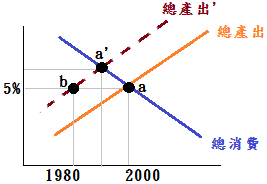
\includegraphics[scale=1.00]{2.png}
\end{figure} 
		\item 若利率不改變,此經濟的總產出少了甲原先可產出的20石,總產出會變成1980石,如上圖點b處。但均衡狀態應為點a',利率會高於5\%,而總產出大於1980石,小於2000石。
	\end{num}
\end{num}

\end{CJK}
\end{document}
